\section{Metric Graphs}
\label{ch1:sec1}

This chapter is dedicated to the introduction of the basic principles about metric graphs and resulting concepts, which we need for a reasonable derivation of numerical methods on these structures. The following material has been adopted from \cite[chapter~1]{BerkolaikoKuchment:2013} unless otherwise noted. \\

We define a graph $\Gamma$ as an ordered pair $(\mathcal{V}, \mathcal{E})$, where $\mathcal{V} = \{v_i\}$ is a finite set of points, which we call vertices, and $\mathcal{E} = \{e_j\}$ is a set of segments connecting some of the vertices, which we call edges. In the following we will use the notation $E \coloneqq \left\lvert \mathcal{E} \right\rvert$ for the number of edges and $V \coloneqq \left\lvert \mathcal{V} \right\rvert$ for the number of vertices. \\
Each edge $e \in \mathcal{E}$ can be identified with a pair $(v, w)$ of vertices $v, w \in \mathcal{V}$, which it connects. An edge $e \in \mathcal{E}$ is called a directed edge if a direction is assigned to it, which means that this edge $e = (v, w)$ can only be followed in one direction. In this case, the order of the pair of vertices $(v, w)$ describing a directed edge $e$ is important. Directed edges are also called bonds, which is why we will denote the set of all directed edges of a graph by $\mathcal{B}$, directed edges with $b \in \mathcal{B}$ and the number of directed edges with $B \coloneqq \left\lvert \mathcal{B} \right\rvert$ in the following. The set of bonds $\mathcal{B}$ can be uniquely described as a set of ordered pairs of vertices $\mathcal{B} = \{b_i\}_{i = 1, \ldots, B} = \{(v^{o}_{i}, v^{t}_{i})\}_{i = 1, \ldots, B}$, where the first vertex $v^{o}_{i}$ is called the origin vertex and the second vertex $v^{t}_{i}$ is called the terminal vertex of the corresponding bond $b_i$. These origin and terminal vertices of a bond can be specified via functions $o \colon \mathcal{B} \to \mathcal{V}$ and $t \colon \mathcal{B} \to \mathcal{V}$, i.e. a bond $b = (v^{o}, v^{t})$ begins at $o(b) = v^{o}$ and ends at $t(b) = v^{t}$. We define the set of incoming bonds at a vertex $v$ as the set of bonds satisfying $t(b) = v$, if $o(b) = v$, the bond $b$ is called outgoing at the vertex $v$. \\
If all edges of a graph $\Gamma = (\mathcal{V}, \mathcal{E})$ are bonds, i.e. $\mathcal{E} = \mathcal{B}$, then we call this graph $\Gamma$ a directed graph. A graph $\Gamma = (\mathcal{V}, \mathcal{E})$ is called non-directed if it does not have any bonds, which means that each of its edges $e \in \mathcal{E}$ can be followed in both directions. In this case, the order of the two connected vertices describing a non-directed edge is unimportant, i.e. $e = (v, w) = (w, v)$ with $v, w \in \mathcal{V}$. \\
In general, graphs are represented as one-dimensional drawings of points and lines, where the points represent the vertices and the lines represent the edges. \cref{fig1:f1} shows an non-directed graph. In a directed graph, an arrow at the end of an edge indicates which direction is assigned to the corresponding edge, as shown in \cref{fig1:f2}. 

\begin{figure}[H]
    \begin{subfigure}[b]{0.4\textwidth}
        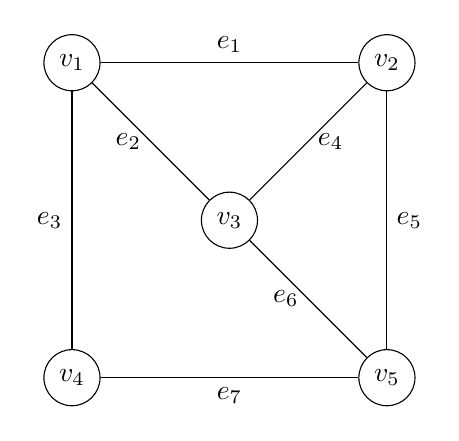
\begin{tikzpicture}
            % vertices
            \node[shape=circle,draw=black] (v1) at (0,4) {$v_1$};
            \node[shape=circle,draw=black] (v2) at (4,4) {$v_2$};
            \node[shape=circle,draw=black] (v3) at (2,2) {$v_3$};
            \node[shape=circle,draw=black] (v4) at (0,0) {$v_4$};
            \node[shape=circle,draw=black] (v5) at (4,0) {$v_5$};
            
            % edges
            \path [-](v1) edge node[above] {$e_1$} (v2);
            \path [-](v1) edge node[left] {$e_2$} (v3);
            \path [-](v1) edge node[left] {$e_3$} (v4);
            \path [-](v2) edge node[right] {$e_4$} (v3);
            \path [-](v2) edge node[right] {$e_5$} (v5);
            \path [-](v3) edge node[left] {$e_6$} (v5);
            \path [-](v4) edge node[below] {$e_7$} (v5);
        \end{tikzpicture}
        \caption{Non-directed graph}
        \label{fig1:f1}
    \end{subfigure}
    \hfill
    \begin{subfigure}[b]{0.4\textwidth}
        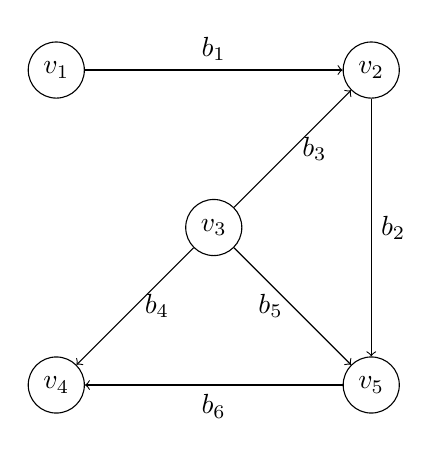
\begin{tikzpicture}
            % vertices
            \node[shape=circle,draw=black] (v1) at (0,4) {$v_1$};
            \node[shape=circle,draw=black] (v2) at (4,4) {$v_2$};
            \node[shape=circle,draw=black] (v3) at (2,2) {$v_3$};
            \node[shape=circle,draw=black] (v4) at (0,0) {$v_4$};
            \node[shape=circle,draw=black] (v5) at (4,0) {$v_5$};
            
            % edges
            \path [->](v1) edge node[above] {$b_1$} (v2);
            \path [->](v2) edge node[right] {$b_2$} (v5);
            \path [->](v3) edge node[right] {$b_3$} (v2);
            \path [->](v3) edge node[right] {$b_4$} (v4);
            \path [->](v3) edge node[left] {$b_5$} (v5);
            \path [->](v5) edge node[below] {$b_6$} (v4);
        \end{tikzpicture}
        \caption{Directed graph}
        \label{fig1:f2}
    \end{subfigure}
    \caption{Two different types of graphs.}
\end{figure}

It is necessary for some considerations that a non-directed graph $\Gamma = (\mathcal{V}, \mathcal{E})$ will be considered as a directed graph by assigning two bonds $b$ and $\overline{b}$ with opposite directions to each edge $e \in \mathcal{E}$ of the non-directed graph $\Gamma$, as shown in \cref{fig2}. We denote the resulting directed graph by $\widetilde{\Gamma} = (\mathcal{V}, \widetilde{\mathcal{E}})$.

\begin{figure}[H]
    \begin{subfigure}[b]{0.4\textwidth}
        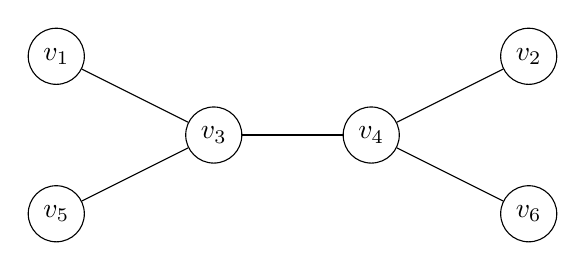
\begin{tikzpicture}
            % vertices
            \node[shape=circle,draw=black] (v1) at (-3,1) {$v_1$};
            \node[shape=circle,draw=black] (v2) at (3,1) {$v_2$};
            \node[shape=circle,draw=black] (v3) at (-1,0) {$v_3$};
            \node[shape=circle,draw=black] (v4) at (1,0) {$v_4$};
            \node[shape=circle,draw=black] (v5) at (-3,-1) {$v_5$};
            \node[shape=circle,draw=black] (v6) at (3,-1) {$v_6$};
            
            % edges
            \path [-](v1) edge (v3);
            \path [-](v5) edge (v3);
            \path [-](v3) edge (v4);
            \path [-](v2) edge (v4);
            \path [-](v6) edge (v4);
        \end{tikzpicture}
        \caption{Non-directed graph $\Gamma$.}
    \end{subfigure}
    \hfill
    \begin{subfigure}[b]{0.4\textwidth}
        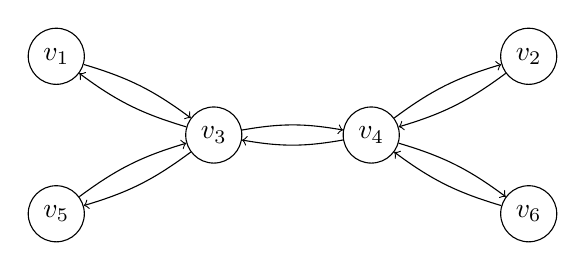
\begin{tikzpicture}
            % vertices
            \node[shape=circle,draw=black] (v1) at (-3,1) {$v_1$};
            \node[shape=circle,draw=black] (v2) at (3,1) {$v_2$};
            \node[shape=circle,draw=black] (v3) at (-1,0) {$v_3$};
            \node[shape=circle,draw=black] (v4) at (1,0) {$v_4$};
            \node[shape=circle,draw=black] (v5) at (-3,-1) {$v_5$};
            \node[shape=circle,draw=black] (v6) at (3,-1) {$v_6$};
            
            % edges
            \path [->](v1) edge [bend left = 10] (v3);
            \path [->](v3) edge [bend left = 10] (v1);
            \path [->](v5) edge [bend left = 10] (v3);
            \path [->](v3) edge [bend left = 10] (v5);
            \path [->](v3) edge [bend left = 10] (v4);
            \path [->](v4) edge [bend left = 10] (v3);
            \path [->](v2) edge [bend left = 10] (v4);
            \path [->](v4) edge [bend left = 10] (v2);
            \path [->](v6) edge [bend left = 10] (v4);
            \path [->](v4) edge [bend left = 10] (v6);
        \end{tikzpicture}
        \caption{Directed graph $\widetilde{\Gamma}$.}
    \end{subfigure}
    \caption{Obtaining a directed graph $\widetilde{\Gamma}$ by duplicating the edges of the non-directed graph $\Gamma$.}
    \label{fig2}
\end{figure}

The graph $\widetilde{\Gamma} = (\mathcal{V}, \widetilde{\mathcal{E}})$ with $\widetilde{\mathcal{E}} = \mathcal{B}$ satisfies the condition that at each vertex $v \in \mathcal{V}$ the numbers of incoming and outgoing bonds are equal, i.e. $\left\lvert \{ b \in \mathcal{B} \, \colon \, o(b) = v \} \right\rvert = \left\lvert \{ b \in \mathcal{B} \, \colon \, t(b) = v \} \right\rvert$. The set of bonds $\mathcal{B}$ is symmetric in the sense that $b \in \mathcal{B}$ if and only if there is another bond $\overline{b} \in \mathcal{B}$ such that $o(b) = t(\overline{b})$ and $t(b) = o(\overline{b})$ holds. The bond $\overline{b}$ is called the reversal of $b$. The operation of reversal is reflexive, i.e. $\overline{\overline{b}} = b$. \\
On a graph $\Gamma = (\mathcal{V}, \mathcal{E})$ is a vertex $w \in \mathcal{V}$ called adjacent to a vertex $v \in \mathcal{V}$, denoted by $v \sim w$, if a suitable edge $e \in \mathcal{E}$ exists, so that $w$ can be reached from $v$ via this edge $e$. In the following we assume that a graph has no loops, which are edges that connect a vertex $v \in \mathcal{V}$ to itself, i.e. $v \sim v$, and no multi-edges, which are several equal edges between two vertices, i.e. $e_1, e_2 \in \mathcal{E}$ and $e_1 = e_2$. \\
A graph $\Gamma = (\mathcal{V}, \mathcal{E})$ with $\mathcal{V} = \{v_i\}_{i = 1, \ldots, V}$ is fully specified by its $V \times V$ adjacency matrix $A^{\Gamma}$. The entries of the adjacency matrix are given by
\begin{equation}
    \label{adjacency matrix}
    A^{\Gamma}_{i, j}= \begin{cases} 1 & \text{if } v_i \sim v_j \\ 0 & \text{otherwise. } \end{cases}
\end{equation}
One sees immediately that the adjacency matrix of an non-directed graph is symmetric, since a vertex $v \in \mathcal{V}$ is adjacent to another vertex $w \in \mathcal{V}$ exactly when the other way round is also true, i.e. $v \sim w \Leftrightarrow w \sim v$. \\
The degree $d_{v_i}$ of a vertex $v_i \in \mathcal{V}$ is the number of edges that are connected to the vertex $v_i$, i.e. $d_{v_i} = \sum_{v_j \in \mathcal{V}} A_{i, j}$. For a directed graph the number of incoming bonds at a vertex $v_i$ is called incoming degree of $v_i$, denoted by $d^{t}_{v_i}$, and the number of outgoing bonds at a vertex $v_i$ is called outgoing degree of $v_i$, denoted by $d^{o}_{v_i}$. Clearly, $d^{t}_{v_i} + d^{o}_{v_i} = d_{v_i}$ holds. All degrees are assumed to be finite and positive, we hence exclude vertices with no edges coming in or going out. We will denote by $D^{\Gamma}$ the degree matrix of a graph $\Gamma = (\mathcal{V}, \mathcal{E})$, which is a diagonal $V \times V$ matrix with the entries
\begin{equation}
    \label{degree matrix}
    D^{\Gamma}_{i, j} = d_{v_i} \, \delta_{v_j, v_i}
\end{equation}
where $\delta_{v_j, v_i}$ is the Kronecker delta. \\
A vertex is incident to an edge, denoted by $v \in e$, if the vertex $v \in \mathcal{V}$ is one of the two vertices the edge $e \in \mathcal{E}$ connects. We define for an non-directed graph $\Gamma = (\mathcal{V}, \mathcal{E})$ with $\mathcal{V} = \{v_i\}_{i = 1, \ldots, V}$ and $\mathcal{E} = \{e_i\}_{i = 1, \ldots, E}$ the $V \times E$ incidence matrix $I^{\Gamma}$ by  
\begin{equation}
    \label{incidence matrix non-directed}
    I^{\Gamma}_{i, j}= \begin{cases} 1 & \text{if } v_i \in e_j \\ 0 & \text{otherwise.} \end{cases}
\end{equation}
For a directed graph $\Gamma = (\mathcal{V}, \mathcal{E})$ with $\mathcal{V} = \{v_i\}_{i = 1, \ldots, V}$ and $\mathcal{E} = \mathcal{b} = \{b_i\}_{i = 1, \ldots, B}$ we define the $V \times B$ incidence matrix $I^{\Gamma}$ by 
\begin{equation}
    \label{incidence matrix directed}
    I^{\Gamma}_{i, j}= \begin{cases} 1 & \text{if } b_j = (v_i, \cdot) \\ -1 & \text{if } b_j = (\cdot, v_i) \\ 0 & \text{if } v_i \notin b_j. \end{cases}
\end{equation}
We further denote by $\mathcal{E}_v$ the set of all edges incident to the vertex $v$ (i.e., containing $v$). \\

So far we have considered graphs as discrete combinatorial objects. From now on we consider graphs as 1-dimensional complexes and the edges will be treated as 1-dimensional segments. For this exists a natural projection $\pi \colon \widetilde{\Gamma} \to \Gamma$ that maps two points $x_b$ and $x_{\overline{b}}$ of bonds $b$ and $\overline{b}$ that are reversals connecting the vertices $v_1$ and $v_2$ to a point $x_e$ on a non-directed edge $e$ connecting the same vertices $v_1$ and $v_2$ as shown in \cref{fig3}.

\begin{figure}[H]
    \begin{center}
        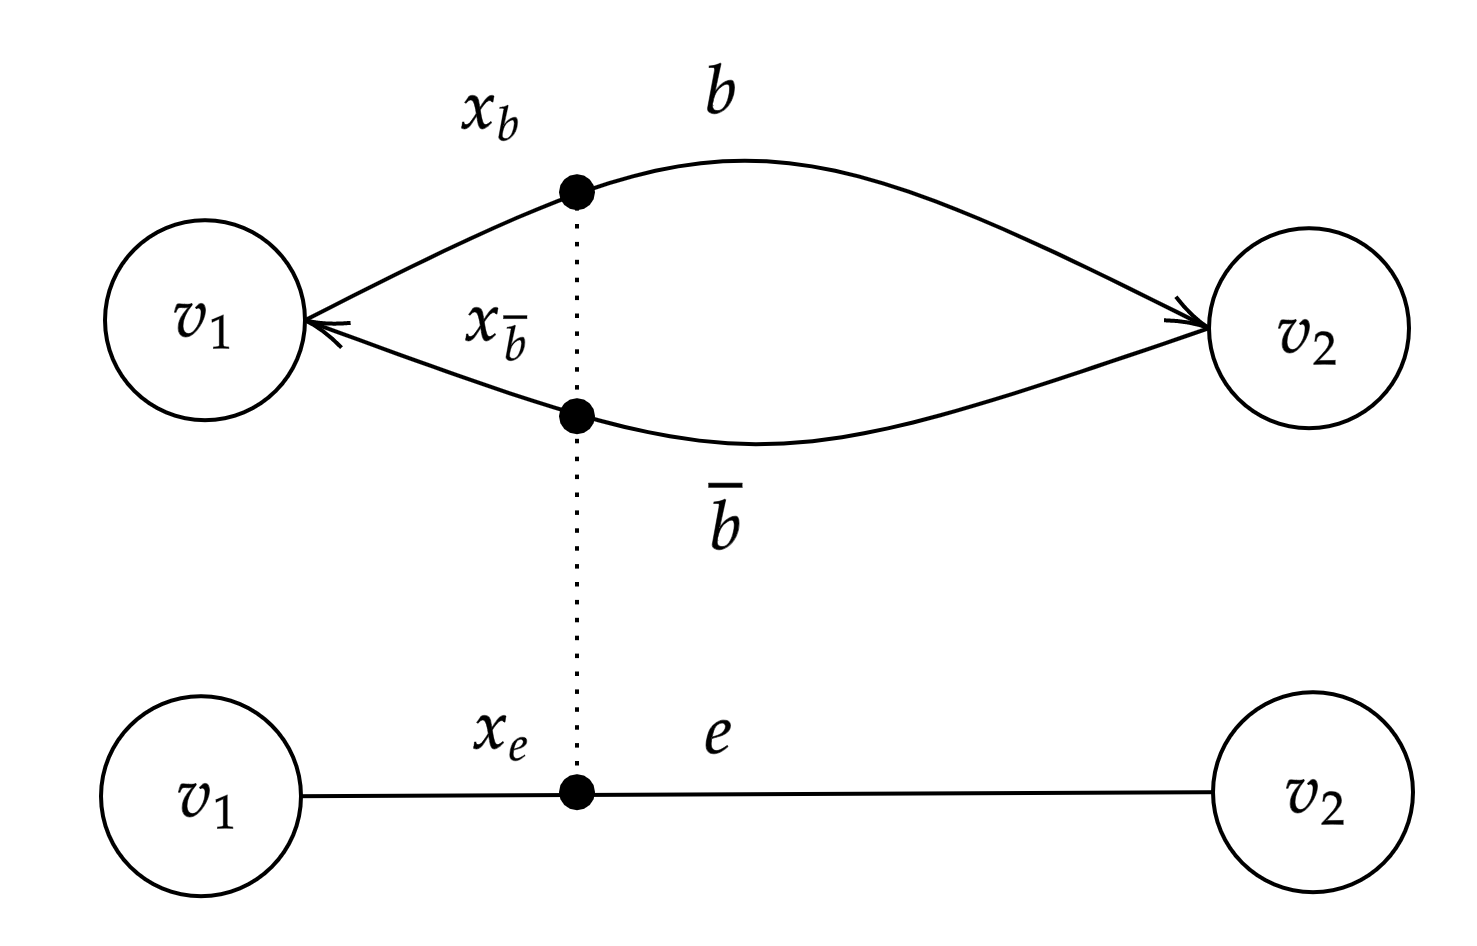
\includegraphics[scale=0.2]{img/diagram-20220201_3.png}
    \end{center}
    \caption{Projection $\pi \colon \widetilde{\Gamma} \to \Gamma$ illustrated on a single edge.}
    \label{fig3}
\end{figure}

Roughly speaking, we now imagine the edges $\mathcal{E}$ of a graph $\Gamma = (\mathcal{V}, \mathcal{E})$ not as abstract relations between the vertices $\mathcal{V}$, but rather as physical “wires” connecting them. For that we add a structure that equips $\Gamma$ with a topology and metric. 

\begin{definition}[{\cite[Definition~1.3.1.]{BerkolaikoKuchment:2013}}]\label{metric graph}
    A graph $\Gamma = (\mathcal{V}, \mathcal{E})$ is said to be a metric graph, if 
    \begin{enumerate}
        \item each bond $b$ is assigned a positive length $l_b \in (0, \infty)$;
        \item the lengths of the bonds that are reversals of each other are assumed to be equal, i.e. $l_b = l_{\overline{b}}$, and thus the length $l_e$ of an edge $e$ is also defined (by the projection $\pi$, see \cref{fig3});
        \item a coordinate $x_b \in [0, l_b]$ increasing in the direction of the bond is assigned on each bond;
        \item the relation $x_{\overline{b}} = l_b − x_b$ holds between the coordinates on mutually reversed bonds (in other words, $x_{\overline{b}}$ and $l_b − x_b$ are mapped to the same point on $e$ by the projection $\pi$, see \cref{fig3}).
    \end{enumerate}
\end{definition}

In most cases, when this does not lead to any confusion, we will drop the subscript of the coordinate $x_b$ and denote it just by $x$. From \cref{metric graph} and \cref{fig3} it is clear that a metric graph can directed or non-irected or it can be a graph $\Gamma = (\mathcal{V}, \mathcal{E})$ that contains both directed and undirected edges, i.e. $\mathcal{B} \subsetneqq \mathcal{E}$. Of course, in the case of a non-directed edge $e = (v, w)$, one must then determine at which of the two vertices $x_e = 0$ and at which $x_e = l_e$ applies. \\
For some considerations it makes sense that the lengths of all edges are equal, which justifies the following notion:

\begin{definition}[{\cite[Definition~1.3.2.]{BerkolaikoKuchment:2013}}]\label{metric graph}
    A metric graph $\Gamma$ is said to be equilateral, if the lengths of all its bonds (equivalently, edges) are equal: $l_b \equiv l$.
\end{definition}

%Having the length assigned, an edge e will be identified with a finite or infinite segment [0, le] of the real line with the natural coordinate xe along it. In most cases we will drop the subscript in the coordinate and call it x, which should not lead to any confusion. This enables one to interpret the graph Γ as a topological space (simplicial complex) that is the union of all edges where the ends corresponding to the same vertex are identified

%So, now one can imagine the graph Γ as a one-dimensional simplicial complex, each 1D simplex (edge) of which is equipped with a smooth structure, with singularities arising at junctions (vertices) 

